%\iffalse
\let\negmedspace\undefined
\let\negthickspace\undefined
\documentclass[journal,12pt,twocolumn]{IEEEtran}
\usepackage{cite}
\usepackage{amsmath,amssymb,amsfonts,amsthm}
\usepackage{algorithmic}
\usepackage{textcomp}
\usepackage{xcolor}
\usepackage{txfonts}
\usepackage{listings}
\usepackage{enumitem}
\usepackage{mathtools}
\usepackage{gensymb}
\usepackage{comment}
\usepackage[breaklinks=true]{hyperref}
\usepackage{tkz-euclide} 
\usepackage{listings}
\usepackage{gvv}                            \usepackage{tikz}
\usepackage{circuitikz}
\def\inputGnumericTable{}                                
\usepackage[latin1]{inputenc}                            
\usepackage{color}                                       
\usepackage{array}                                       
\usepackage{longtable}                                   
\usepackage{calc}                              
\usepackage{tikz}
\usepackage{multirow}                                    
\usepackage{hhline}                                      
\usepackage{ifthen}                            
\usepackage{caption}
\usepackage{lscape}
\usepackage{amsmath}
\newtheorem{theorem}{Theorem}[section]
\newtheorem{problem}{Problem}
\newtheorem{proposition}{Proposition}[section]
\newtheorem{lemma}{Lemma}[section]
\newtheorem{corollary}[theorem]{Corollary}
\newtheorem{example}{Example}[section]
\newtheorem{definition}[problem]{Definition}
\newcommand{\BEQA}{\begin{eqnarray}}
\newcommand{\EEQA}{\end{eqnarray}}
\newcommand{\define}{\stackrel{\triangle}{=}}
\theoremstyle{remark}
\newtheorem{rem}{Remark}

\begin{document}

\bibliographystyle{IEEEtran}
\vspace{3cm}

\title{GATE 2021 EE.20}
\author{EE23BTECH11010 - VENKATESH BANDAWAR$^{*}$% <-this % stops a space
}
\maketitle
\newpage
\bigskip
\textbf{Question:} The Bode magnitude plot for the transfer function $\frac{V_o(s)}{V_i(s)}$ of the circuit is as shown. The value of R is \_\_\_\_\_$\Omega$. \hfill(GATE 2021 EE Q20)
\begin{figure}[!ht]
    \centering
    \begin{circuitikz}
   \draw(0,0) to [R](2,0);
   % \draw (2,0) -- (2.5,0);
   \draw(2,0) to [L] (4,0);
   % \draw (5,0) to (5,0);
   \draw (4,0) to [C] (4,-2);
   \draw(4,-2)  to (0,-2);
   \draw (4,0) -- (5,0);
   \draw (4,-2)to (5,-2);
   \node[circle,fill,inner sep=1pt] at (0,0) {};
   \node[circle,fill,inner sep=1pt] at (5,0) {};
   \node[circle,fill,inner sep=1pt] at (5,-2) {};
   \node[circle,fill,inner sep=1pt] at (0,-2) {};
   \draw[->](0,-1.85) to (0,-0.15);
   \draw[->](5,-1.85) to (5,-0.15);
   \node at (0.3,-1) {$V_i$};
   \node at (5.5,-1) {$V_o$};

   \node at (1,0.5) {$R$};
   \node at (3,0.5) {$1mH$};
   \node at (2.8,-1) {$250\micro F$};\node[circle,fill,inner sep=1pt] at (0,0) {};
\end{circuitikz}

\end{figure}
\begin{figure}[!ht]
    \centering
    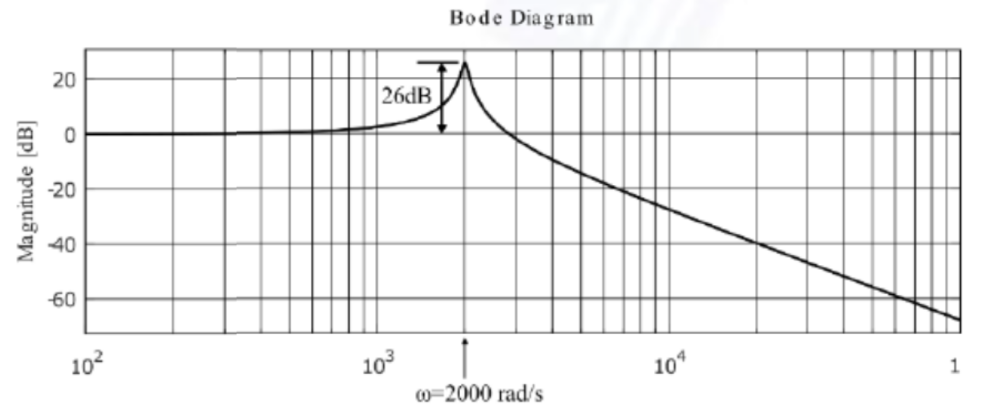
\includegraphics[width=\columnwidth]{figs/bode.png}
\end{figure}
\solution
\begin{table}[!ht]
    \centering
    \begin{tabular}{|c|c|c|}
\hline
    Parameter & Description & Value\\
    \hline
    $P(s)$ & Plant Transfer Function & $\frac{0.001}{s\brak{\frac{s}{0.5}+1}\brak{\frac{s}{100}+1}}$\\
    \hline
    $C(s)$ & Lag Compensator  & $\frac{100\brak{\frac{s}{10}+1}}{\frac{s}{0.1}+1}$\\
    \hline
    $T(s)$ & Loop gain  & $P(s) C(s)$ \\
    \hline
    $\omega$ & Angular Frequency & 3rad/s \\
    \hline
\end{tabular}

    \caption{Given Parameters table}
    \label{Given Parameters table_2021_EE_20}
\end{table}
Applying KVL,
\begin{align}
    V_i - R I - L\frac{dI}{dt} - \frac{\int I dt}{C} = 0
\end{align}
Taking Laplace Transform ,
\begin{align}
    V_i(s) &- RI(s) - LsI(s) + LI(0^+) - \frac{I(s)}{sC} = 0\\
    I(s) &= \frac{V_i(s) + LI(0)}{R + sL + \frac{1}{sC}}\\
    V_o(s) &= \frac{V_i(s) + LI(0)}{RsC + s^2LC + 1}
\end{align}
Substituting $I(0) = 0$ and $s = j\omega$,
\begin{align}
    \frac{V_o(j\omega)}{V_i(j\omega)} &= \frac{1}{\omega RCj -\omega^2LC + 1} 
\end{align}
$\because$ Magnitude in bode plot = $20\log \abs{T(s)}$\\
From given graph,At $\omega = 2000$
\begin{align}
    26 &= 20 \log \abs{\frac{V_o}{V_i}}\\
    \abs{\frac{V_o}{V_i}} &= 20
\end{align}
\begin{align}
    \implies 20 &= \abs{\frac{1}{\omega RCj -\omega^2LC + 1}} \\
    R &= 0.1 \Omega
\end{align}
\begin{figure}[!h]
    \centering
    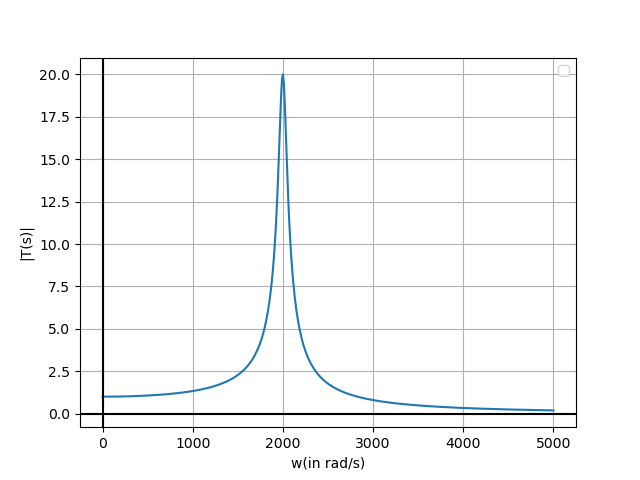
\includegraphics[width=\columnwidth]{figs/frequency_response.png}
    \caption{Frequency response of $V_o$}
    \label{frequency_response_2021_EE_20}
\end{figure}
\end{document}
